% exercise sheet with header on every page for math or close subjects
\documentclass[12pt]{article}
\usepackage{german} 
\usepackage[utf8]{inputenc} 
\usepackage{latexsym} 
\usepackage{multicol}
\usepackage{fancyhdr}
\usepackage{amsfonts} 
\usepackage{amsmath}
\usepackage{amssymb}
\usepackage{enumerate}
\usepackage{MnSymbol}
\usepackage[colorlinks=true,urlcolor=blue]{hyperref}
\usepackage{listings}
\usepackage{graphicx}

% Shortcuts for bb, frak and cal letters
\newcommand{\E}{\mathbb{E}}
\newcommand{\V}{\mathbb{V}}
\renewcommand{\P}{\mathbb{P}}
\newcommand{\N}{\mathbb{N}}
\newcommand{\R}{\mathbb{R}}
\newcommand{\C}{\mathbb{C}}
\newcommand{\Z}{\mathbb{Z}}
\newcommand{\Pfrak}{\mathfrak{P}}
\newcommand{\Pfrac}{\mathfrak{P}}
\newcommand{\Bfrac}{\mathfrak{P}}
\newcommand{\Bfrak}{\mathfrak{B}}
\newcommand{\Fcal}{\mathcal{F}}
\newcommand{\Ycal}{\mathcal{Y}}
\newcommand{\Bcal}{\mathcal{B}}
\newcommand{\Acal}{\mathcal{A}}


% Formatierung
\topmargin -2cm 
\textheight 24cm
\textwidth 16.0 cm 
\oddsidemargin -0.1cm

\setlength{\parindent}{0pt}  % !!!!!!! Hier werden leerzeilen erlaubt ohne dass Latex automatisch einrueckt! !!!!!!! %


%Python code Highlighting
\lstset{language=Python, tabsize=3,
        basicstyle=\ttfamily\small, 
        keywordstyle=\color{keywords},
        commentstyle=\color{comments},
        stringstyle=\color{red},
        showstringspaces=false,
        identifierstyle=\color{green}}

% Code-Highlighting Java
%\lstset{language=Java, breaklines=true, showstringspaces=false}
%\begin{lstlisting}
%    	Hier würde der Java-Code hinkommen und entsprechend die Syntax markiert. Selbst einrücken.
%\end{lstlisting}
%ODER:
% \lstinputlisting[language=Java]{name.py}

\graphicspath{ {images/} }


\begin{document}

% Titel
%\title{\textsc{Hacking}\\ \textsc{Abgabe 0}\\{ \normalsize Gruppe X \hfill Daniel Schäfer (2549458)\\ \hfill Anderer}}
%\maketitle  

% alternativer Titel
\noindent
{\Large \textbf{High-level Computer Vision}} \hfill \textbf{26.05.2016}\\
{\Large \textbf{Exercise 3}} 
\raggedleft \hfill Guillermo Reyes (2556018)\\
\hfill Daniel Schaefer (2549458)\\
\hfill Marc Tonsen (2537359)\\
\hfill Dominik Weber (2548553)\\

\pagenumbering{gobble}
\raggedright


\section*{Code Annotations}




\section*{Question 1: Support Vector Machines}

\begin{enumerate}[a)]
	\setcounter{enumi}{1}
	\item 	
        \textbf{Modify the last two parameters of} \verb!get\_train\_dataset\_2d.m! \textbf{in order to make the classification problem linearly non-separable. Run your visualization for different values of parameter C and comment on its role in the SVM classification algorithm.}\\
        
        	\begin{figure}[h]			
        		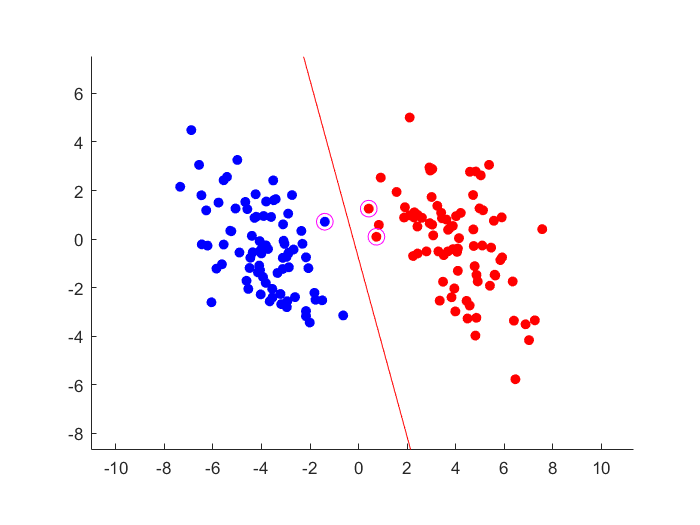
\includegraphics[width=0.5\textwidth]{1b_separable}
        		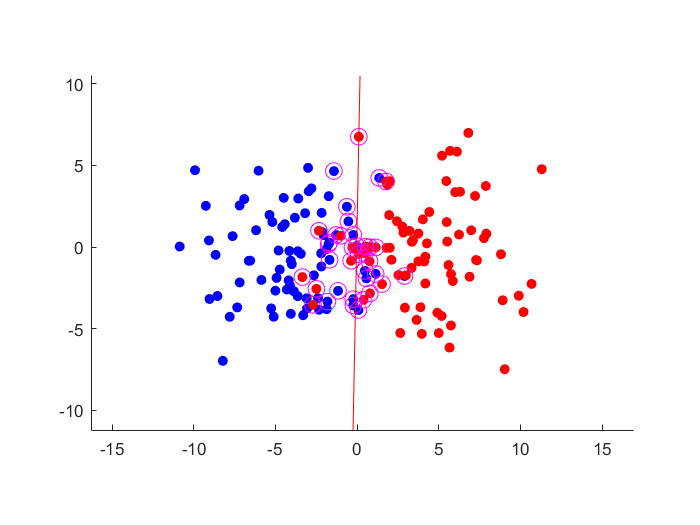
\includegraphics[width=0.5\textwidth]{1b_non-separable}
        		\caption{\textit{Left}: SVM for linearly separable data with default parameters. $ \sigma_1=1.5, \sigma_2=5 $  . \textit{Right}: SVM for linearly non-separable data. The same parameters are used to generate the data except that $ \sigma_1=10 $ and $\sigma_2=10 $ }
        	\end{figure}
        
		The parameter C is used in the minimized loss function to tune the importance of the sum of $\xi$'s. A high value for C would put a lot of importance on them and would therefore force them to take very small values. Therefore, the higher the value of C is, the closer the performance comes to that of a hard-margin SVM. If C has a small value this would soften the margin and would also allow support vectors that are further further away from the margin. In conclusion C influences how soft the margin of the SVM is.
\end{enumerate}

\newpage
\section*{Question 3: Performance Evaluation}
\begin{enumerate}[a)]
	\setcounter{enumi}{3}
	

	\item
        \textbf{Write a summary of your observations and submit it along with the corresponding RPC curves}\\
        %TODO

	\item 
        \textbf{How could you use the system to solve the detection problem in which you are given an image of arbitrary size and the task is to find the position of the people in it?}\\
        %TODO

\end{enumerate}


\end{document}
